\documentclass[11pt]{scrartcl}

\usepackage[hidelinks, colorlinks=true]{hyperref}

\usepackage[english]{babel}
\usepackage{helvet}
\usepackage{mathpazo}
\usepackage{euler}
\usepackage{scrlayer-scrpage}
\usepackage[authoryear]{natbib}
\usepackage{csquotes}
\usepackage{xcolor}
\definecolor{@darkblue}{RGB}{0,0,140}
\definecolor{@darkgreen}{RGB}{0,100,70}
\hypersetup{
	colorlinks   = true, %Colours links instead of ugly boxes
	urlcolor     = @darkblue, %Colour for external hyperlinks
	linkcolor    = @darkblue, %Colour of internal links
	citecolor    = @darkgreen %Colour of citations
}
\usepackage[all]{hypcap}
\usepackage{subcaption}


\usepackage{amsmath}
\usepackage{amsfonts}
\usepackage{amssymb}
\usepackage{adjustbox}

\usepackage{mathtools}
\usepackage{epigraph}
\usepackage{setspace}
\usepackage{listings}
\usepackage{algorithm}
\usepackage{algpseudocode}

\usepackage{tikz, pgfplots}
\usetikzlibrary{calc,decorations.pathmorphing,patterns, pgfplots.colorbrewer, shapes, arrows}
% Define block styles
\tikzstyle{decision} = [diamond, draw, fill=blue!20, 
text width=4.5em, text badly centered, node distance=3cm, inner sep=0pt]
\tikzstyle{block} = [rectangle, draw, fill=blue!20, 
text width=6em, text centered, rounded corners, minimum height=4em]
\tikzstyle{cheap} = [rectangle,  
text width=12em, text centered, minimum height=4em, node distance=3cm]
\tikzstyle{line} = [draw, -latex']
\tikzstyle{cloud} = [draw, ellipse,fill=red!20, node distance=3cm,
minimum height=2em]


% ----------------- Layout stuff  -------------------------------

\pagestyle{scrheadings}
\clearscrheadfoot
%\automark{section}
%\renewcommand\sectionmark[1]{\markright{\MakeMarkcase {\thesection\hskip .5em\relax#1}}\rohead{\ifnum\expandafter\pdfstrcmp\botmark=0 \rightmark\else\leftmark{} --- \rightmark\fi}}


\ofoot{\pagemark}

% ---------------------  Title page setup ----------------------------
% Title Page
\title{Minimal Surfaces}
\author{add your matriculation numbers here!\\Chenfei Fan \\  Praveen Mishra \\ Sankarasubramanian Ragunathan\\ Philipp Schleich\quad 391779}
%
\subject{Report \\ Simulation Sciences Laboratory}
\date{\today \\ \vspace{0.9cm}}

\publishers{
	\vspace{2em}
	
	\begin{tabular}[!b]{ll}
		Supervisor: & Prof. Dr. Uwe Naumann \\[3pt]
		            & Klaus Leppkes
	\end{tabular}
%	\begin{figure}[h!]
%		\centering
%		\includegraphics[width=.6\linewidth]{figs/mathccesText.png}%
%		
%	\end{figure}
}
% -------------------------------------------------------------

\newcommand{\mSurf}[1]{\ensuremath{\mathcal{F}\left[#1\right]}}
\newcommand{\mSurfDisc}[1]{\ensuremath{\mathtt{F}^h\left[#1\right]}}
\newcommand{\Dx}[1]{\ensuremath{\mathtt{d}_x[#1]}}
\newcommand{\Dy}[1]{\ensuremath{\mathtt{d}_y[#1]}}
\newcommand{\Dxx}[1]{\ensuremath{\mathtt{d}_{xx}[#1]}}
\newcommand{\Dyy}[1]{\ensuremath{\mathtt{d}_{yy}[#1]}}
\newcommand{\Dxy}[1]{\ensuremath{\mathtt{d}_{xy}[#1]}}

\newcommand{\inv}{\ensuremath{^{-1}}}

\begin{document}
\maketitle

%\section*{Abstract}
%\begin{abstract}
%\noindent Abstract might be unnecessary
%\end{abstract}
%
\clearpage
\protect \tableofcontents



\newpage
	
\onehalfspacing
% #########################################################################
\section{Introduction}
@Sankar, sth like in the presentation
% #########################################################################
\section{Background}
\subsection{General background (don't like this title)}
We look at surfaces in $ \mathbb{R}^3 $, defined over an open set $\Omega \subset \mathbb{R}^2$. 
The surface of desire should contain the least possible area among all possible surfaces, that assume given values on the boundary of $\Omega$, denoted by $\partial \Omega$. \cite{Sakai1976}

Lagrange showed in 1760, that such a surface is characterized by the graphic of a function $z(x,y)$, $z: \mathbb{R}^2 \to \mathbb{R} $, which is twice continuously differentiable on a twodimensional domain, particularly in a subset of $\mathbb{R}^2$.
This function $z$ has to fulfill the so called \textit{Minimal-Surface Equation} (MSE) stated below.
\begin{align}\label{eq:MSE}
	(1+z_y^2) z_{xx} - 2 z_x z_y z_{xy} + (1+z_x^2)z_{yy} = \mSurf{z} &= 0 \quad &\text{in } \Omega \\
	z(x,y) &= g(x,y) \quad &\text{on } \partial \Omega \notag
\end{align}
Clearly, this formulation satisfies the prescribed boundary values given by $g(x,y)$ due to the Dirichlet boundary condition on $\partial\Omega$.
As to why the graphic of functions solving this equation describes a minimal surface, we refer to the literature. For example \cite{Sakai1976} gives a very straightforward proof.

In the following, we will call the differential operator $\mSurf{\cdot}$ the Minimal-Surface Operator (MSO). The resulting partial differential equation (PDE) in eq. \eqref{eq:MSE} turns out to be an elliptic PDE of second order, which is in particular \textit{non-linear}. The solution of such a PDE is not trivial, and typically requires numerical treatment. For certain cases, analytical descriptions are available, such as for Scherk's surface.

\begin{figure}
	\centering
	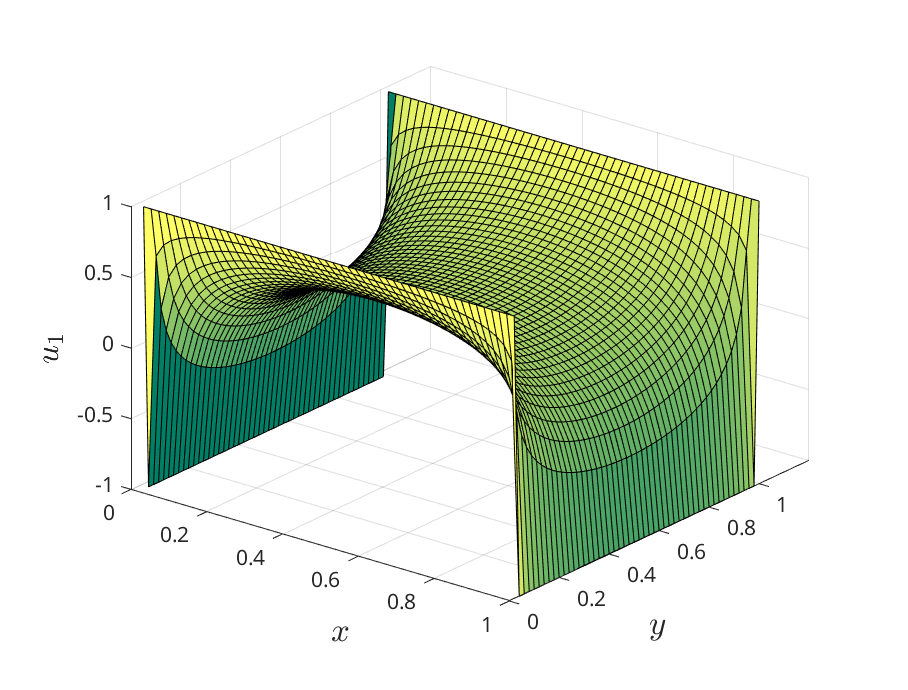
\includegraphics[width=.5\textwidth]{figs/scherk-test}
	\caption{Scherk's first surface on $[0,1]^2$}\label{fig:scherk01}
\end{figure}


\newpage

As an example, Scherk's first surface (compare to figure \ref{fig:scherk01}) $\Sigma$ rescaled on $\Omega = [0,1]^2$ is given by
\begin{equation}
	\Sigma = \left\{ \left. \left(x, y, \log \left( \frac{\cos (\pi(x-\frac{1}{2}))}{\cos (\pi(y-\frac{1}{2}))} \right) \right) \in \mathbb{R}^{3} \right  | 0 < x, y < 1 \right\}.
\end{equation} 
which is the limit $n\to \infty$ of 
\begin{align}
\Sigma_n = \left\{ \left. \left(x, y, u_n(x,y) \right) \in \mathbb{R}^{3} \right  | 0 < x, y < 1 \right\}, \\
\lim\limits_{y\to \pm 1} \to n \quad, 0 \le x \le 1 \\
\lim\limits_{x\to \pm 1} \to -n \quad, 0 \le y \le 1.
\end{align}


The numerical solution of the MSE will require setting approbiate boundary conditions. Since $\log \left( \frac{\cos (\pi(x-\frac{1}{2}))}{\cos (\pi(y-\frac{1}{2}))} \right) \to \pm \infty $ on $\partial\Omega$, this is numerically not very practical. 

We thus introduce $\beta_x,\beta_y \in (0,1)$ s.th. 
\begin{equation}
\Sigma_{\text{trunc}} = \left\{ \left. \left(x, y, \log \left( \frac{\cos (\pi\beta_x(x-\frac{1}{2}))}{\cos (\pi\beta_y(y-\frac{1}{2}))} \right) \right) \in \mathbb{R}^{3} \right  | 0 < x, y < 1 \right\}.
\end{equation} 

By these means, we solve the MSE on $\Omega_\text{trunc}=[0,1]^2\subset\Omega$ with $\Omega=[0,\frac{1}{\beta_x}]\times[0,\frac{1}{\beta_y}]$. Exact boundary values on $\partial\Omega_\text{trunc}$ ensure the correctness of the results. We choose $\beta_x=\beta_y=\beta$, as we restrict ourselves to solving on a square domain.

Later on, we will use this surface as a test-case to verify our numerical results.

\newpage
\subsection{Numerical solution}
\subsubsection{Discretization}
In this project, we are supposed to solve the MSE numerically on $\Omega \equiv (0,1)\times(0,1)$. In the following, discretized quantities are indicated by a superscript $h$. The spatial domain is to be discretized using a structured mesh with equidistant grid spacing both in $x,y$, i.e. we have the same number of grid points in both directions, $N=N_x=N_y$. Thus, we define $\Omega^h := \{ (x,y) \in \mathbb{R}^2:\text{ }(x,y) = (ih, jh), \text{ } 0 \le i,j < N,\text{ }hN=1\}$.

\begin{figure}[h!]
	\centering
	\adjustbox{scale=3}{ 
	\begin{tikzpicture}
	\draw [gray!50!white, step=0.2] (-0.3,-0.3) grid (1.3,1.3);
	\draw [thick, ->] (0,-0.4) -- (0,1.4);
	\draw [thick, ->] (-0.4,0) -- (1.4,0);
	
	\draw [red, thick] (0,0) rectangle (1,1);
	
	\node at (-0.17,-0.14) [scale=0.4] {(0,0)};		
	\node at (1.17,-0.14) [scale=0.4] {(1,0)};		
	\node at (-0.17,1.1) [scale=0.4] {(0,1)};		
	\node at (1.17,1.1) [scale=0.4] {(1,1)};	
	\node at (-.55, .7) [blue, scale=.5] {$\Omega^h$};	
	\node at (-.4, .45) [red, scale=.5] {$\partial\Omega^h$};	
	
	
	
	% Boundary nodes
	\foreach \x in {0,1,2,3,4,5} {
		\foreach \y in {0} { % bottom
			\node at (\x/5,\y/5) [circle,fill=red, scale=0.3] {};
			%this way circle of nodes will not be transformed
		}
	}
	\foreach \x in {0} { % left
		\foreach \y in {0, 1,2,3,4,5} {
			\node at (\x/5,\y/5) [circle,fill=red, scale=0.3] {};
			%this way circle of nodes will not be transformed
		}
	}
	\foreach \x in {0,1,2,3,4,5} { % top
		\foreach \y in {5} {
			\node at (\x/5,\y/5) [circle,fill=red, scale=0.3] {};
			%this way circle of nodes will not be transformed
		}
	}
	\foreach \x in {5} { % right
		\foreach \y in {0,1,2,3,4,5} {
			\node at (\x/5,\y/5) [circle,fill=red, scale=0.3] {};
			%this way circle of nodes will not be transformed
		}
	}
	%Inner nodes
	\foreach \x in {1,2,3,4} {
		\foreach \y in {1,2,3,4} {
			\node at (\x/5,\y/5) [circle,fill=blue, scale=0.3] {};
			%this way circle of nodes will not be transformed
		}
	}
	\end{tikzpicture}
	}
	\caption[Depiction of $\Omega^h$ with $N=5$, $hN=1$]{Depiction of $\Omega^h$ with $N=5$, $hN=1$. Blue: inner nodes, red: boundary nodes}
\end{figure}

We choose to discretize the MSO on $\Omega^h$ by Finite Differences, since this is usually the easiest way to go, and on a structured grid, would anyways yield similar discrete equation as in Finite Volume or Finite Element methods.

To obtain a second order consistent discrete MSO (\mSurfDisc{\cdot}), we use central difference stencils on the first, second and mixed derivative. Since all these stencils have make only use of immediate neighours, there is no need to treat nodes close to the boundary differently, since the boundary is given by $g(\cdot)$.

This way, we obtain a discrete version of \eqref{eq:MSE}:
\begin{align}
	\left(1+\Dx{z^h}^2\right)\Dyy{z^h}-\Dx{z^h} \Dy{z^h}\Dxy{z^h} + \left(1+\Dy{z^h}^2\right)\Dxx{z^h} = \mSurfDisc{z^h} &= 0  \quad \text{in } \Omega^h \notag \\
	z^h &= g \quad \text{on } \partial\Omega^h \label{eq:dMSE},
\end{align}
while the stencils defined on the inner nodes are given as follows ($1 \le i,j \le N-1$):
\begin{align}
	\Dx{z} &= \frac{z_{i+1,j}-z_{i-1,j}}{2h} \\
	\Dy{z} &= \frac{z_{i,j+1}-z_{i,j-1}}{2h} \\
	\Dxx{z} &= \frac{z_{i+1,j} - 2z_{i,j} + z_{i-1,j}}{h^2}\\
	\Dyy{z} &= \frac{z_{i,j+1} - 2z_{i,j} + z_{i,j-1}}{h^2}\\
	\Dxy{z} &= \frac{z_{i+1,j+1} + z_{i-1,j-1} - z_{i-1,j+1}-z_{i+1,j-1}}{4h^2}. 
\end{align}
Figure~\ref{fig:fdmmesh} depicts the stencils on a segment of $\Omega^h$.
Since the stencils have only support to the nearest neighbors, there is no need tho treat nodes close to the boundary any different. Furthermore, this gives already rise to the conclusion, that the associated matrix will be sparse (for each of the $N$ gridpoints, only 9 instead of $N$ partners contribute).

\begin{figure}
	\centering
	\includegraphics[width=.4\linewidth]{figs/FDMMesh}
	\caption{Snippet of the mesh with Finite Differences stencils\\red/blue: first and second order stencils in $x,y$\\
	green: mixed stencil}\label{fig:fdmmesh}
\end{figure}
\newpage
\subsubsection{Solution}
The main difficulty in solving the MSE lies in the non-linearity of $\mSurfDisc{\cdot}$. Since it is not possible, to directly invert for $z^h = \left(\mathtt{F}^h\right)\inv 0$, one needs to use a procedure such as Newton-Raphson iterations. The main idea is to use some initial guess $z^h_0$, while in general, $\mSurfDisc{z^h_0}=r^h_k\neq0$. The goal is then to generate a sequence of $z^h_k$ such that $r^h_k\to 0$ for increasing, but reasonably small $k$. Algorithm~\ref{algo:standard-newton} shows the standard Newton-Raphson procedure, that takes as input a specific initial guess (here: 0), a tolerance for convergence \textsc{tol} and the nonlinear operator $\mSurfDisc{\cdot}$, outputting an approximate solution to the MSE $z^h_{k_\text{fin}}$.
\begin{algorithm}
	\caption{Newton's method applied on the discrete MSE}\label{algo:standard-newton}
	\begin{algorithmic}
		\State $k \gets 0$ 
		\State $z^h_k \gets 0 $ 
		\State $r^h_k \gets \mSurfDisc{z^h_k}$
		\While{$\lVert r^h_k \rVert > \textsc{tol}$} \Comment{ We choose $ \lVert \cdot \rVert = \lVert \cdot \rVert_2  $}
			\State $z^h_{k+1} \gets z^h_{k} - \left(\nabla\mSurfDisc{z^h_k}\right)\inv r^h_k $
			\State $k \gets k+1$ 
			\State $r^h_k \gets \mSurfDisc{z^h_k}$
		\EndWhile
	\end{algorithmic}
\end{algorithm}

This algorithm involves the computation of the inverse of the gradient of $\mSurfDisc{z^h_k}$ for each iteration $k$. Later, we will present and compare two different ways on how to contrive this.

It is well known, that the Newton-Raphson procedure yields fast convergence, but the success of this convergence is highly dependent on the initial guess $z^h_0$. Furthermore, convergence can be improved by choosing an initial guess that is closer to the solution. 
One possible initial guess is to take the average boundary value, \\$z^h_{0,\text{ave}}=\frac{1}{|\partial\Omega^h|} \sum_{(x_i,y_j)\in \partial\Omega^h} \big(g(x_i,y_j)\big)$. While this might help convergence for surfaces, that have a certain offset with respect to the $x,y$-plane, it does not provide any additional information (such as preshaping curvature).

To obtain a more educated initial guess, recall the MSE, equation \eqref{eq:MSE}. Considering only linear terms, we get 
\begin{align}
	\mathcal{L} [z] = z_{xx} + z_{yy} &= 0 \quad\quad\quad\quad \text{ in } \Omega \\
	z(x,y) &= g(x,y) \quad \text{ on } \partial\Omega \notag 
\end{align}\newpage
This linear, second order PDE is well known as the Laplace-equation, and can be solved by discretizing the second derivatives using the definitions for $\Dxx{\cdot},\Dyy{\cdot}$ introduced before, yielding $\mathtt{L}[z^h]=0 $ with the usual boundary conditions. Since Laplace's equation can be regarded as a linearization of the MSE, we suspect to get a better initial guess (and thus faster and a more robust convergence behaviour) by first solving for $z^h_0= \mathtt{L}\inv 0$. This way, we obtain a slightly modified version of Algorithm~\ref{algo:standard-newton}, stated in Algorithm~\ref{algo:laplace-newton}.

\begin{algorithm}
	\caption{Newton's method using Laplace's Equ. as initial guess}\label{algo:laplace-newton}
	\begin{algorithmic}
		\State $k \gets 0$ 
		\State $z^h_k \gets \mathtt{L}\inv 0 $ \Comment{Solve Laplace's Equ. as initial guess}
		\State $r^h_k \gets \mSurfDisc{z^h_k}$
		\While{$\lVert r^h_k \rVert > \textsc{tol}$} 
		\State $z^h_{k+1} \gets z^h_{k} - \left(\nabla\mSurfDisc{z^h_k}\right)\inv r^h_k $
		\State $k \gets k+1$ 
		\State $r^h_k \gets \mSurfDisc{z^h_k}$
		\EndWhile
	\end{algorithmic}
\end{algorithm}

\clearpage
\subsection{Consequences for a implementation}
So far we discussed the abstract numerical setting to solve the MSE. But when implementing this as a software solution, one has to consider several additional points, which especially involve the interface to the user.

\begin{figure}[b]
	\centering
	\begin{tikzpicture}[node distance=4cm, auto]
	% Place nodes
	\node [block] (code) {Code/Solver};
	\node [cloud, left of=code, node distance=3cm] (in) {user input};
	\node [cloud, right of=code, node distance=3.5cm] (out) {output to user};
	%
	\path [line] (in) -- (code);
	\path [line] (code) -- (out);
	
	\node [cheap, below of=in](inputLegend) at(-3.8,0.3) {
		\small\begin{itemize}
		\item mesh size 
		\item boundary conditions 
		\item \dots
		\end{itemize}
		$\rightarrow$ user interface \\ via input file \normalsize
	};
	
	\node [cheap, below of=code] (solverLegend) at(0,0.25) {%
		\small\begin{itemize}
		\item discretization/grid 
		\item apply BC 
		\item determine Jacobian 
		\item solve linear systems 
		\item Newton iterations  \normalsize
		\end{itemize}
	};
	
	\node [cheap, below of = out] (outLegend) at(3.8, 0.3) {
		\small\begin{itemize}
		\item visualization of solution 
		\item convergence output (residual) 
		\item check validity of result
		\end{itemize}\normalsize
	};
	\end{tikzpicture}
	\caption{Requirements on a potential implementation}
\end{figure}
% #########################################################################
\section{Implementation}

How we implemented things, ...

\subsection{Software/Solver Design}
@Sankar, here the UML chart + explain the "flow"

either change the name of "Dependencies" of make sure to explain it like during the Q\&A-session

\subsection{Computing the Jacobian}
@Chenfei, briefly explain like in the presentation the three methods, and also name that one could use Finite Differences, but this is expected to perform bad (because...), and thus we do not use it (the next lines are already a few months old, use them or get rid of them)

Within the Newton iterations, it is necessary to compute the inverse of the Jacobian of the discrete MSO. We implemented this procedure following two different strategies:
\begin{itemize}
	\item Based on generating the Jacobian matrix $\nabla\mSurfDisc{z^h_k}$ and computing its inverse
	\begin{itemize}
		\item Hard-code a manually calculated Jacobian (to verify results)
		\item Build a Jacobian matrix from Automatic Differention (AD by hand)
	\end{itemize}
	\item Based on a linear iterative scheme, where we do not explicitly build the Jacobian, but extract its action on certain vectors from AD and feed this to a linear iterative solver
\end{itemize}

Argue that, since $\nabla F$ is not symmetric in general, need stabilized CG (better performance than GMRES according to Eigen library)


		\begin{algorithm}[H]
			\caption{Newton's method}
			\begin{algorithmic}
				\State $y \gets \mathtt{F}(z)$ 
				\While{$\lVert y \rVert > \textsc{tol}$} 
				\State $A = \nabla \mathtt{F}(z)$ 
				\State \color{blue} $dz = A\inv y$  \normalcolor \Comment{Instead of assembling the whole $\nabla \mathtt{F}$ above, do this matrix-free}
				\State $z \gets z + dz$
				\State $\mathtt{res} \gets \mathtt{F}(z)$ 
				\EndWhile
			\end{algorithmic}
		\end{algorithm}
		\begin{algorithm}[H]
			\caption{Matrix-free BiCGSTAB to get $dz$ (adapted from \cite{naumann})}
			\small{	\begin{algorithmic}
					\State $z^{(1)} \gets dz$ 
					\State \color{blue}$(y, y^{(1)}) \gets \mathtt{F}^{(1)} (z, z^{(1)}) $ \normalcolor \Comment{DCO}
					\State $p \gets -y -y^{(1)}$
					\State $r \gets p, r_0\gets r, \rho\gets1,\alpha\gets1,\omega\gets1 $
					\While{$\lVert r \rVert > \textsc{tol}$} 
					\State $\rho_{\text{new}} = \big(r_0,r\big)$
					\State $z^{(1)} \gets p$
					\State $\beta \gets \rho_{\text{new}}/\rho \cdot \alpha/\omega$
					\State $\rho \gets \rho_{\text{new}}$
					\State $p\gets r+\beta(p-\omega v)$
					\State $z^{(1)} \gets p$
					\State \color{blue}$(y, y^{(1)}) \gets \mathtt{F}^{(1)} (z, z^{(1)}) $ \normalcolor \Comment{DCO}
					\State $\alpha \gets \rho/\big(r_0,y^{(1)}\big)$ 
					\State $dz \gets dz + \alpha p$
					\State $s\gets r - \alpha y^{(1)}$
					\State $z_1 \gets z + dz$
					\State \color{blue}$(y_1, y_1^{(1)}) \gets \mathtt{F}^{(1)} (z_1, z_1^{(1)}) $ \normalcolor \Comment{DCO}
					\If{$\lVert y_1 \rVert < \textsc{tol} $}
					\State abort \Comment{Converged at intermediate level}
					\EndIf
					\State $z^{(1)} \gets s$
					\State \color{blue}$(y, y^{(1)}) \gets \mathtt{F}^{(1)} (z, z^{(1)}) $ \normalcolor \Comment{DCO}
					\State $\omega \gets \big(y^{(1)}, s \big) / \big(y^{(1)}, y^{(1)} \big)$
					\State $dz \gets dz + \omega s$
					\State $r \gets s - \omega y^{(1)}$
					\State $z \gets z + dz$
					\EndWhile
			\end{algorithmic}}
		\end{algorithm}


\subsection{Solving linear systems}

	\textbf{I tested a bit now, and will push also to the code, timings ideally after that:
	seems like sparseLU is faster for getting the initial guess, so I will implement that.\\
	for the loops, bicgstab is still advantageous as we can greatly reduce TOL\_linsolver.}
\normal
\subsection{Testing}
@Praveen
here the figure as in the presentation, short explanation (basically what you said)

maybe 1-2 results of tests, short explanation

checking of validity by means of scherk, present a result here

% #########################################################################
\section{Results}
@Praveen you can refer to Scherk from General background, 
results for the 2 testcases, some timings (for all solvers for a choice of $\#$gridpoints, not too many), scaling of the three (fix $\#$gridpoints to sth $>500$ for jacOption 0,1 and maybe max. 200-300 for 2, and run for 1,2,4,8,16 threads)
once timings are implemented, you can also ask us to help determine times (consistent TOL's etc...)


% #########################################################################
\section{Conclusions and outlook}
pretty much what we had in the presentation

@all, feel free to add ideas here, I would merge it together in the end

% #########################################################################

%
\bibliography{bibliography}

\appendix
\section{User manual @Philipp}
short explanation of the params inthe input file, and how to run simulations

\end{document}          
